\section{Das C++ Interface}
\label{sec:cxx_interface}

\projectname{} ermöglicht eine sehr einfache Integration des Lispinterpreters in bestehende C++-Projekte. Sowohl Objekte als auch Funktionen können sehr einfach der Lispseite bekannt gemacht werden.

\subsection{C++ Funktionen an \projectname{} übergeben}
\label{sec:cxx_function_interface}

Jede Funktion, die an \projectname{} übergeben werden soll muss als Methode einer von !object! abgeleiteten Klasse realisiert werden. Der !operator()! wird dabei überschrieben; als Argumente bekommt die Methode eine Referenz auf die aktuelle Umgebung\footnote{Näheres in Abschnitt \ref{sec:environment}.} sowie eine Liste übergebener Parameter. Diese sind noch nicht evaluiert, um beispielsweise die Implementierung einer if-Funktion zu ermöglichen. Die Liste selber ist --- lisptypisch ---
eine Verkettung von !cons_cell!s. 
\begin{figure}[htbp]
\centering
\captionabove{Eigene Funktionen von object ableiten}
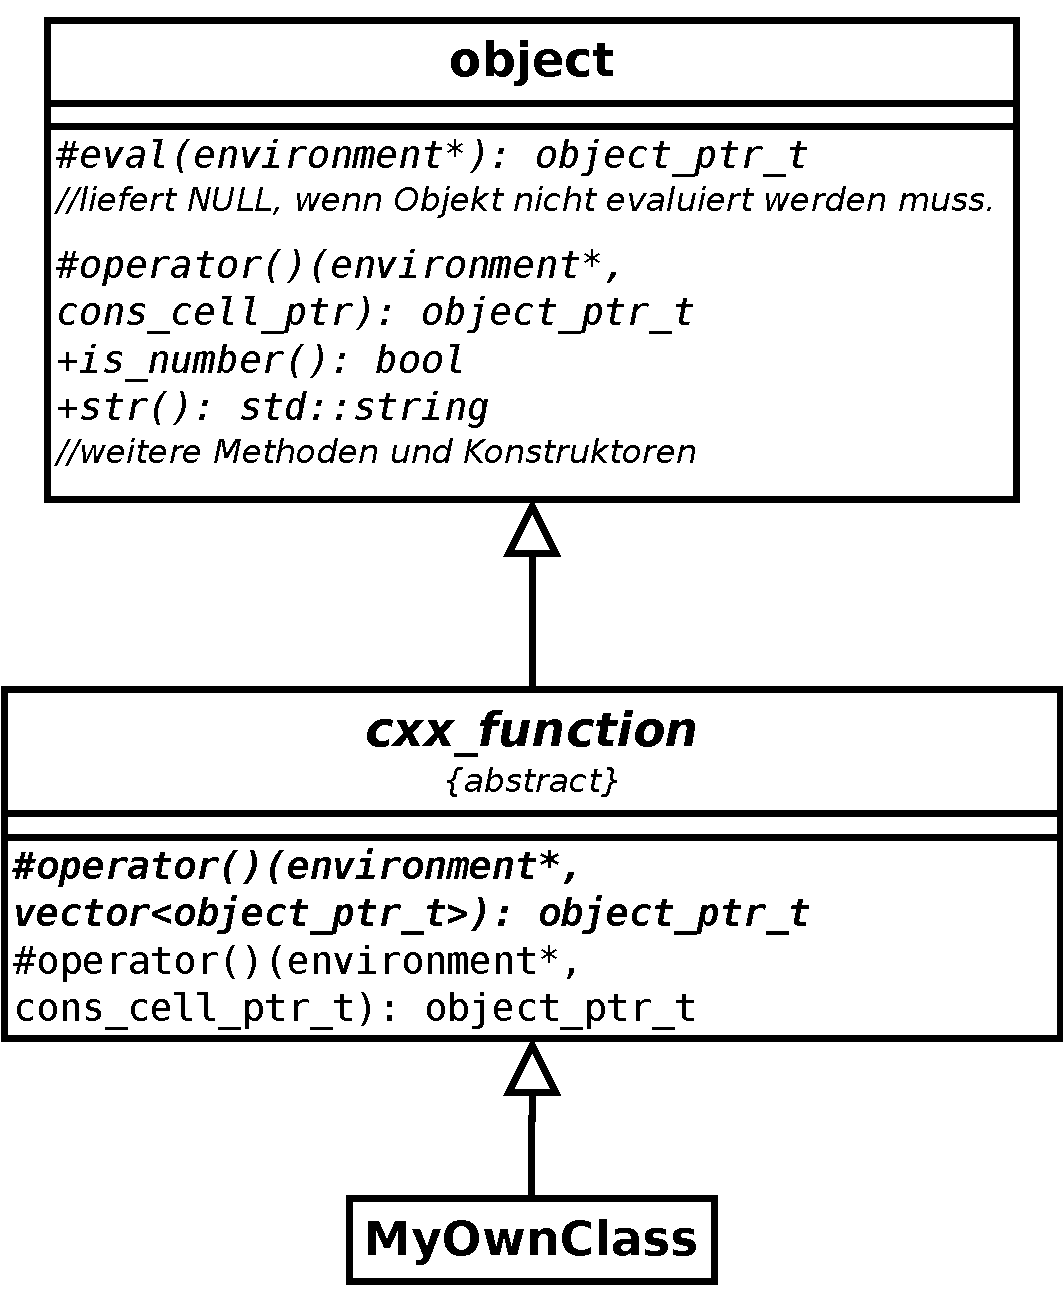
\includegraphics[width=0.5\textwidth]{images/cxx_interface.pdf}
\label{fig:cxx_interface}
\end{figure}
Zur einfacheren Handhabung in eigenen Funktionen existiert jedoch auch die Klasse !cxx_function!. Diese übernimmt das Evaluieren und die Umwandlung der Parameterliste in einen !vector!. Nur die Anzahl und der Typ der Parameter muss noch überprüft werden. Konkret bedeutet dies, dass jede übergebene Funktion den !operator()! einer von !cxx_function! abgeleiteten Klasse überschreibt und dann eine Instanz dieser Klasse an \projectname{} übergeben wird (Abbildung \ref{fig:cxx_interface}). Zur Typprüfung der Parameter existiert für Zahlen die Methode !is_number!; andere Typen, beispielsweise von C++ Seite übergebene, müssen mithilfe der RTTI überprüft werden. Als Beispiel dienen in Listing \ref{lst:cxx_function} die arithmetischen Operatoren.
\begin{lstlisting}[caption={Arithmetische Operatoren an Lisp übergeben}, label=lst:cxx_function]
template <template <typename Type> class Operator,
          char OpName>
class arith_op_form : public cxx_function
{
    object_ptr_t operator()(environment* env,
                            const argv_t& args)
        {
            size_t sz = args.size();
            if(sz <= 1)
                signal(env->get_symbol(
                           "wrong-number-of-arguments"),
                       to_string(OpName));
            if(!args[0]->is_number())
                signal(env->get_symbol(
                           "wrong-type-argument"),
                       to_string(OpName) + ": numberp "
                                         + args[0]->str());

            number_ptr_t res = 
                boost::dynamic_pointer_cast<lisp::number>(
                args[0]);

            for(unsigned int i = 1; i < sz; i++)
            {
                if(args[i]->is_number())
                {
                    number_ptr_t num =
                        boost::dynamic_pointer_cast
                            <lisp::number>(args[i]);
                    Operator<number> op;

                    *res = op(*res, *num);
                }
                else
                    signal(env->get_symbol(
                               "wrong-type-argument"),
                           to_string(OpName) + ": numberp "
                                         + args[i]->str());
            }

            return res;
        }
};

//in lisp.cpp: lisp::*global_env()

_global_env.get_symbol("+")->set_function(
    object_ptr_t(new arith_op_form<std::plus, '+'>()));
_global_env.get_symbol("-")->set_function(
    object_ptr_t(new arith_op_form<std::minus, '-'>()));
_global_env.get_symbol("*")->set_function(
    object_ptr_t(new arith_op_form<std::multiplies, '*'>()));
_global_env.get_symbol("/")->set_function(
    object_ptr_t(new arith_op_form<std::divides, '/'>()));
\end{lstlisting}

\subsection{C++-Objekte an \projectname{} übergeben}
\label{sec:cxx_object_interface}

C++-Objekte können auf ebenso einfache Weise an die Lispseite übergeben werden wie Funktionen. Die entsprechenden Klassen müssen nur von !object! abgeleitet werden. Erzeugt werden können die Objekte in übergebenen Funktionen um als Rückgabewert auf Lispseite weiterverwendet zu werden. Die Zerstörung der Objekte übernimmt der Garbage Collector (Abschnitt \ref{sec:shared_ptr}). Werden eigene Objekte an Lispfunktionen übergeben, findet wie bereits erwähnt keine automatische Typprüfung statt. Der Typ eines Objekts kann jedoch jeweils mittels des !typeid! Operators bestimmt werden.
%Hier noch ein Beispiel oder so?!

\subsection{Liste unterstützter Formen}
\begin{itemize}
\item !lambda!: Form zum Erstellen anonymer Funktionen.
\item !if!: Verzweigung.
\item !or!: 
\end{itemize}